\begin{enumerate}[label=\thechapter.\arabic*,ref=\thechapter.\theenumi]
\item Let y\brak{t}=x\brak{4t},where x\brak{t} is a continous-time periodic signal of $100$s.the fundamental period of y\brak{t} is (\textbf{rounded off to the nearest integer})
 \hfill(GATE IN 2023)\\
\solution
\newpage
\item In the circuit shown below, it is observed that the amplitude of voltage across the resistor is the same as the amplitude of the sorce voltage. What is the angular frequency $\omega_0$(in rad$/s$)?\\

\begin{circuitikz}[american]
    \draw (0,0) to[R, l=$10K\Omega$] (2,0) to[L, l=$10mH$] (4,0) to[C, l=$1\mu{F}$] (6,0) -- (6,-1) 
    to[sV, l=$100\cos(\omega_0 t)$] (0,-1) -- (0,0)
    (0,-1) node[circ]{} node[left]{$+$}
    (6,-1) node[circ]{} node[right]{$-$};
\end{circuitikz} \hfill(GATE BM 2023)
\solution
\newpage

\item For a regular sinusoidal wave propagating in deep water having wave height of 3.5 m and wave period of 9 s, the wave steepness is \underline{\hspace{1cm}} (round off to three decimal places).
\hfill Gate 2023 NM 33
\solution
\newpage

\item  A spring mass system is shown in the figure . Take the value of acceleration  due to gravity as $g=9.81$ $m/s^2$.The static deflection due to weight and the time period of the oscillations,respectively,are\\\hfill{(GATE 2023 XE)}
 \begin{figure}[h!]
    \centering
    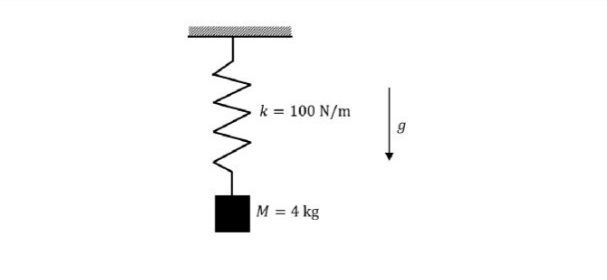
\includegraphics[width = \columnwidth]{2023/XE/71/figs/fig1.jpg}
\end{figure}
\solution

\end{enumerate}
